% Basic preamble
\documentclass[a0paper,landscape,columns=2]{../includes/tex/baposter}

% Pull from header includes


\usepackage[font=small,labelfont=bf]{caption} % specifying captions to tables/figures
\usepackage{booktabs}                         % Horizontal rules in tables
\usepackage{relsize}                          % make text smaller in some places
\usepackage{tipa}
\usepackage{amssymb}
\usepackage{multirow}
\usepackage{multicol}
\usepackage{tikz}
\usepackage[margin=.7cm]{caption}
\usepackage{hhline}
\usepackage{colortbl}


\usetikzlibrary{arrows,decorations.pathmorphing,backgrounds,positioning,fit,matrix,trees,mindmap,shapes}

\graphicspath{{../includes/figs/}} % Directory in which figures are stored

% RU colors
% RU red	RGB 204,0,51

\definecolor{bordercol}{RGB}{0,33,71} % Border color of content boxes
\definecolor{headercol1}{RGB}{204,0,51} % bg color for header in content boxes (left side)
\definecolor{headercol2}{RGB}{204,0,51} % bg color for header in content boxes (right side)
\definecolor{headerfontcol}{RGB}{255,255,255} % Text color for header text in content boxes
\definecolor{boxcolor}{RGB}{255,255,255} % bg color for content in the content boxes
\definecolor{uared}{RGB}{204,0,51}

\usepackage{enumitem}
\setlist{itemsep=.25ex}


% Allow syntax highlighting for r code












\begin{document}




\background{
\begin{tikzpicture}[remember picture,overlay]
  \draw (current page.north west)+(-2em,2em) node[anchor=north west]
  {
\includegraphics[height=1.1\textheight, width=1.1\textwidth]{../includes/figs/white}};
\end{tikzpicture}
  }

\begin{poster}{
  grid=false,
  borderColor=bordercol,         % Border color of content boxes
  headerColorOne=headercol1,     % bg color for header in content boxes (l side)
  headerColorTwo=headercol2,     % bg color for header in content boxes (r side)
  headerFontColor=headerfontcol, % Text color for header text in content boxes
  boxColorOne=boxcolor,          % bg color for content in content boxes
  headershape=roundedright,      % Specify rounded corner in content box headers
  headerfont=\Large\sf\bf,       % Font modifiers for text in content box headers
  textborder=rectangle,
  background=user,
  headerborder=closed,           % Set to closed for a line under content box headers
  boxshade=plain
}
{}
%
% TITLE AND AUTHOR NAME -------------------------------------------------------
%
{
 \sf\bf 
 \phantom{.} \\ 
 \vspace{0.4in}
 \LARGE{White Hmong Reciprocals and Reflexives}}
{
 \vspace{.4em} 
 \textbf{Quartz Colvin} \\ 
 \smaller{Rutgers University \\ New Brunswick, NJ, U.S.A.} \\
 {\vspace{-0.4in}\hspace{-10.40in}
  
\includegraphics[scale=0.3]{../includes/figs/ru_shield2}\phantom{.}} \\
 {\vspace{-0.20in}\smaller quartz.colvin@rutgers.edu} \\
 {\vspace{-0.9in}\hspace{11.05in}
   
\includegraphics[scale=0.3]{../includes/figs/uni-graz.png}\phantom{.}}
}



%
% INTRODUCTION ----------------------------------------------------------------
%

\headerbox{Introduction}{name=introduction,column=0,row=.1}{

\vspace{.1in}

In this project, I provide data from two native speakers to show how reciprocals and reflexives are constructed and bound in White Hmong. I argue that White Hmong follows the traditional binding theory (\cite{reinhart1983}; \cite{chomsky1986}) and supports that $v$P and CP are phases in Hmong. I also show that the true reciprocal is a Voice head (not a DP) in Hmong and the `false’ reciprocal is a reflexive construction with dual or plural pronouns.

\vspace{.25in}

Empirically, Hmong has been understudied and most literature of the language are from the 1900s, so this project is a more modern view of how the language is used by immigrant communities and their children in the United States today.

\vspace{.25in}

}



%
%   FACTS -------------------------------------------------------
%

\headerbox{Facts}{name=facts,column=0,below=introduction}{

\vspace{.1in}

\textbf{Fact 1:} The standard structure of reflexive DPs in Hmong is [Pro + Clf + $kheej$] (1-2)

\vspace{.1in}

\textbf{Fact 2:} $kheej$ `self’ can occur alone as the object of a clause and bind to the subject (3).

\vspace{.1in}

\textbf{Fact 3:} There are two ways to translate reciprocal meanings into Hmong.

\vspace{.1in}

\begin{itemize}

\item[A.] Method 1 is another $kheej$-reflexive construction using a dual pronoun (5).

\vspace{.1in}

\item[B.] Method 2 is a `true reciprocal’ where the reciprocal $sib$ is a Voice morpheme and not a nominal (4,6)

\end{itemize}

\vspace{.1in}

}




\headerbox{Data}{name=data,column=1,row=.1}{
    \begin{itemize}
        \item[(1)] kuv pom kuv tus kheej \\
            \textsc{1sg} see \textsc{1sg} \textsc{Clf} self \\ 
            \textit{"I see myself."}
            \vspace{.05in}
        \item[(2)] nws pom nws tus kheej \\
            \textsc{3sg} see \textsc{3sg} \textsc{Clf} self \\
            \textit{"He sees himself"}
            \vspace{.05in}
        \item[(3)] kuv pom kheej \\
            \textsc{1sg} see self \\
            \textit{"I see myself."}
            \vspace{.05in}
        \item[(4)] lawv sib txawb pob zeb \\
            \textsc{3pl} \textsc{Recip} throw \textsc{Clf} rock \\
            \textit{"They threw rocks at each other."}
            \vspace{.05in}
        \item[(5)] nkawm tham txog nkawm tus kheej \\
            \textsc{3du} talk about \textsc{3du} \textsc{Clf} self \\
            \textit{"They (du.) are talking about each other."}
            \vspace{.05in}
        \item[(6)] nkawm sib tham \\ 
            \textsc{3du} \textsc{Recip} talk \\
            \textit{"They (du.) are talking to each other.}
    \end{itemize}
}


\headerbox{Proposal for Reflexives}{name=reflexive,column=1,below=data}{

\vspace{.1in}

The clausal projection in Hmong is AspP instead of IP or TP since it does not mark tense and is an analytic language (see \cite{lin2006} for Mandarin).

\vspace{.2in}

The subject raises from Spec,$v$P to Spec,AspP due to a strong EPP on Asp \cite{chomsky1982}.

Binding domains are synonymous with phases \cite{chomsky1995}, so binding between the antecedent (in Spec,$v$P) and the reflexive (the sister of V) happens at the $v$P phase (7). The reflexive can either be $kheej$ or a full reflexive DP.

\vspace{.15in}

}



\headerbox{Proposal for Reflexives}{name=reflexives,column=2,row=.1}{

\vspace{.1in}

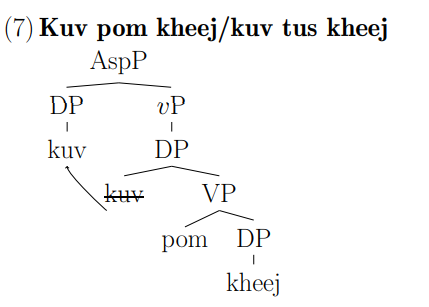
\includegraphics[width=.8\linewidth]{tree7.png}

\vspace{.1in}

I argue that the word $sib$ is a Voice head and not an anaphoric DP

\vspace{.1in}

The word order poses no issues for the SVO word order’s syntax.

\vspace{.1in}

It’s not novel to associate Voice with reciprocity \cite{kratzer1996}, although this has never been discussed with Hmong data.

\vspace{.2in}

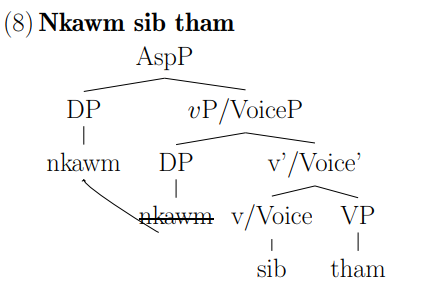
\includegraphics[width=.8\linewidth]{tree8.png}
}

\headerbox{Acknowledgements}{name=acknowledgements,column=2,below=reflexives}{
\begin{small}
I'd like to acknowledge the guidance of Dr. Messick at Rutgers University and my two consultants Keng and Ying Xiong.
\end{small}
}


\headerbox{Proposal for reciprocals}{name=reciprocals,column=3,row=.1}{

\vspace{.1in}

The final structure, (9), shows that the SVO word order truly is maintained when we have both $sib$ and a DP object

\vspace{.1in}

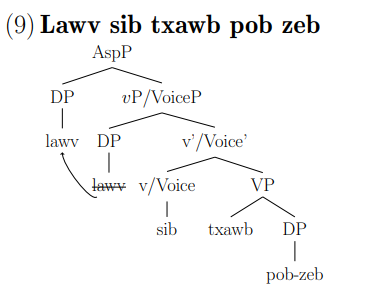
\includegraphics[width=0.60\linewidth]{tree9.png}

\vspace{.1in}

The domain of the reciprocal meaning is the phase.

\vspace{.1in}

Before the subject raises out of the $v$P structure, it is established as the
agent of the reciprocal action.

\vspace{.1in}

Not only is the domain of the reciprocal clear, but the timing of the reciprocal mapping is also clear.

\vspace{.05in}

}





%
%   RESULTS ---------------------------------------------------------------------
%




%
%   CONCLUSION ------------------------------------------------------------------
%











%
%   REFERENCES ------------------------------------------------------------------
%

\headerbox{References}{name=references,column=3,below=reciprocals}{
\begin{small}

% \smaller % Reduce the font size in this block
\renewcommand{\section}[2]{\vskip 0.05em} % Get rid of the default "References" section title
% \nocite{*} % Insert publications even if they are not cited in the poster

\bibliographystyle{unsrt}
\bibliography{../includes/bib/IEEEabrv,../includes/bib/SpeePros} % Use sample.bib as the bibliography file
\end{small}
}


%
%   ACKNOWLEDGEMENTS ------------------------------------------------------------
%




\end{poster}


\end{document}
